% Afficher des recommendations concernant la syntaxe.
\RequirePackage[orthodox,l2tabu]{nag}
\RequirePackage{luatex85}
% Paramètres du document.
\documentclass[%
a3paper%                       Taille de page.
,fontsize=47pt%                Taille de police.
,DIV=17%                       Plus grand => des marges plus petites.
,titlepage=off%                Faut-il une page de titre ?
,headings=optiontoheadandtoc%  Effet des paramètres optionnels de section.
,headings=small%
,parskip=false%
,openany%
]{scrbook}
\renewcommand*\partheademptypage{\thispagestyle{empty}}

%\usepackage{geometry}

% Par souci de clarté, la définition des commandes est reportée dans un document annexe.
\usepackage{gredoc,mudoc,lyluatex}
\usepackage{pdfpages,transparent,array,ltablex}
\addtolength{\voffset}{2mm}\addtolength{\headsep}{-2mm}
\setlength{\extrarowheight}{2mm}
\addto\captionsfrench{%
  \renewcommand{\indexname}{Index des chants}%
}

\pdfcompresslevel=9

\newcommand{\lieu}[1]{\hfill\linebreak[3]\hspace*{\stretch{1}}\nolinebreak\mbox{\emph{(#1)}}}

\newcommand{\commandement}[1]{\noindent\textbf{#1}}

\newcommand{\schola}[1]{}\newcommand{\foule}[1]{#1}
\providecommand{\dest}{foule}

\newcommand{\bgimage}[1]{%
\raisebox{-.45\paperheight}[0pt][0pt]{%
  \transparent{0.3}%
  \includegraphics[width=.7\paperwidth,height=.7\paperheight,keepaspectratio=true]{img/#1}%
  }%
}

\def\arraystretch{1.2}


\grechangedim{overhepisemalowshift}{.7mm}{scalable}
\grechangedim{hepisemamiddleshift}{1.4mm}{scalable}
\grechangedim{overhepisemahighshift}{2.1mm}{scalable}
\grechangedim{vepisemahighshift}{2.1mm}{scalable}

\title{Cantus}
\date{}

\def\blindsection#1{\markright{#1}\addcontentsline{toc}{section}{#1}}

%\pagestyle{empty}

%\includeonly{Parties/Kyriale-XI}

\begin{document}

\thispagestyle{empty}

%{\centering \textbf{Kyriale I}\par}

\bigskip

\cantus{Kyriale}{Kyrie-I}{}{8.}

\cantus{Kyriale}{Gloria-I}{}{4.}

\cantus{Kyriale}{Sanctus-I}{}{4.}

\cantus{Kyriale}{Agnus-I}{}{4.}

%\cantus{Kyriale}{Ite-XI}{}{1.}

%{\centering \textbf{Kyriale II}\par}

\bigskip

\cantus{Kyriale}{Kyrie-II}{}{3.}

\cantus{Kyriale}{Gloria-II}{}{1.}

\cantus{Kyriale}{Sanctus-II}{}{1.}

\cantus{Kyriale}{Agnus-II}{}{1.}

%\cantus{Kyriale}{Ite-XI}{}{1.}

%{\centering \textbf{Kyriale IV}\par}

\bigskip

\cantus{Kyriale}{Kyrie-IV}{}{1.}

\cantus{Kyriale}{Gloria-IV}{}{4.}

\cantus{Kyriale}{Sanctus-IV}{}{8.}

\cantus{Kyriale}{Agnus-IV}{}{6.}

%{\centering \textbf{Kyriale XI}\par}

\bigskip

\cantus{Kyriale}{Kyrie-XI}{}{1.}

\pagebreak[3]
\cantus{Kyriale}{Gloria-XI}{}{2.}

{%
\grechangedim{spacelinestext}{2.8ex}{scalable}
\cantus{Kyriale}{Sanctus-XI}{}{2.}

\grechangedim{spaceabovelines}{1.5ex}{scalable}
\cantus{Kyriale}{Agnus-XI}{}{1.}%
}

%\cantus{Kyriale}{Ite-XI}{}{1.}

%{\centering \textbf{Credo I}\par}

\bigskip

\cantus{Kyriale}{Credo-I}{}{4.}

%{\centering \textbf{Feria VI.\\Quatuor Temporum Adventus}\par}

\bigskip


\cantus{Introit}{PropeEsTu}{Intr.}{4.}

\cantus{Graduel}{OstendeNobis}{Grad.}{2.}

\cantus{Offertoire}{DeusTuConvertens}{Off.}{4.}

\cantus{Communion}{EcceDominusVeniet}{Comm.}{6.}

%{\centering \textbf{In Epiphania Domini}\par}

\bigskip

{%
\gresetinitiallines{2}
\greillumination{\raisebox{2ex}{\hspace{-1ex}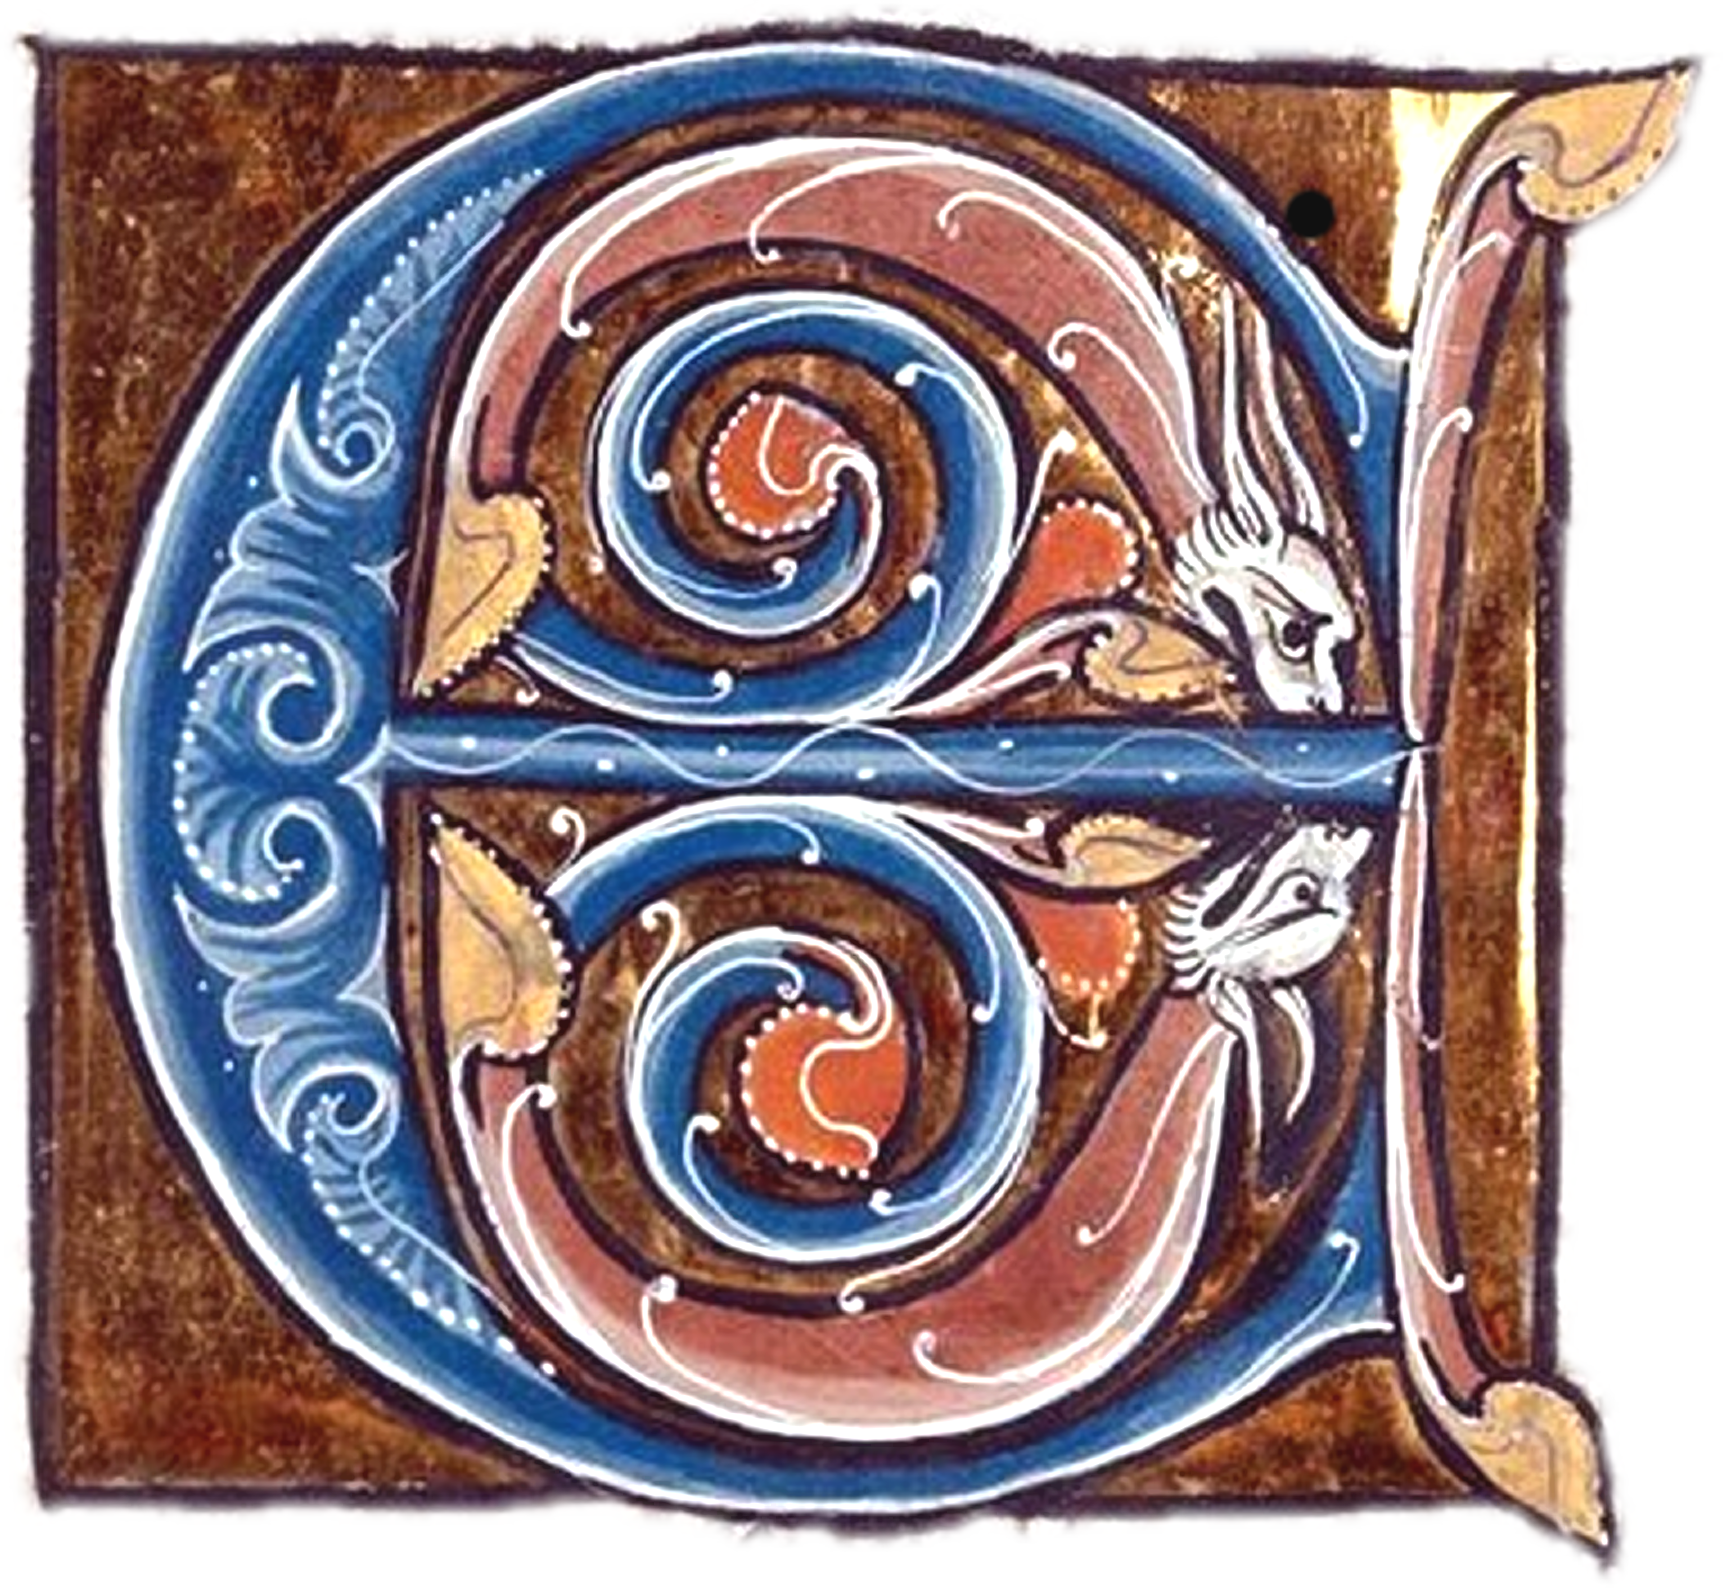
\includegraphics[height=12ex]{img/E0001}}}
\cantus{Introit}{EcceAdvenit}{Intr.}{2.}%
}

\cantus{Graduel}{OmnesDeSaba}{Grad.}{5.}

\cantus{Alleluia}{VidimusStellam}{}{2.}

%\pagebreak
\cantus{Offertoire}{RegesTharsis}{Off.}{5.}

\cantus{Communion}{VidimusStellam}{Comm.}{4.}

%{\centering \textbf{Dominica III. post Epiphaniam}\par}
\chead{Dominica III. post Epiphaniam}

\bigskip

\cantus{Introit}{AdorateDeum}{Intr.}{7.}%

\cantus{Graduel}{TimebuntGentes}{Grad.}{5.}

\cantus{Alleluia}{DominusRegnavit_Exsultet}{}{8.}

\cantus{Offertoire}{DexteraDomini}{Off.}{2.}

\cantus{Communion}{MirabanturOmnes}{Comm.}{7.}

%{\centering \textbf{Dominica in Sexagesima}\par}

\bigskip

{%
\grechangedim{spacelinestext}{2.8ex}{scalable}
\grechangedim{spaceabovelines}{1.5ex}{scalable}
\cantus{Introit}{Exsurge}{Intr.}{1.}%
}%

\cantus{Graduel}{SciantGentes}{Grad.}{1.}

\cantus{Trait}{Commovisti}{Tract.}{8.}

{%
\grechangedim{spacelinestext}{2.8ex}{scalable}
\grechangedim{spaceabovelines}{1.5ex}{scalable}
\cantus{Offertoire}{PerficeGressus}{Off.}{4.}%
}

\cantus{Communion}{Introibo}{Comm.}{8.}

%{\centering \textbf{SS. Fabiani Papæ\\ et Sebastiani Mart.}\par}
\chead{\rubrum Festa Ianuarii. 20.}

\bigskip

\cantus{Introit}{IntretInConspectu}{Intr.}{4.}

\cantus{Graduel}{GloriosusDeus}{Grad.}{1.}

\needspace{.3\paperheight}
\cantus{Alleluia}{SanctiTui_Benedicent}{}{2.}

\cantus{Offertoire}{Laetamini}{Off.}{1.}

\cantus{Communion}{Multitudo_AdEum}{Comm.}{2.}

%{\centering \textbf{In Cathedra S. Petri Apostoli}\par}
\chead{\rubrum Festa Februarii. 22.}

\bigskip

\cantus{Introit}{Statuit}{Intr.}{1.}

\needspace{.5\paperheight}
\cantus{Graduel}{ExaltentEum}{Grad.}{5.}

\needspace{.3\paperheight}
\cantus{Alleluia}{TuEsPetrus}{}{2.}

\cantus{Trait}{TuEsPetrus}{Tract.}{2.}

\needspace{.3\paperheight}
\cantus{Offertoire}{TuEsPetrus}{Off.}{1.}

\needspace{.3\paperheight}
\cantus{Communion}{TuEsPetrus}{Comm.}{6.}

{\centering \textbf{Commemoratio Beatæ Mariæ Virginis\\ de Monte Carmelo}\par}
\chead{\rubrum Festa Iulii. 16.}

\bigskip

{%
\gresetinitiallines{2}
\grechangedim{beforeinitialshift}{0pt}{scalable}
\grechangedim{afterinitialshift}{0pt}{scalable}
\greillumination{\raisebox{1em}{
\includegraphics[width=10\cm]{G}}}
\cantus{Introit}{Gaudeamus_MariaeVirginis_lettrine}{Intr.}{1.}%
}

\needspace{.3\paperheight}
\cantus{Graduel}{Benedicta}{Grad.}{4.}

\cantus{Alleluia}{PerTeDeiGenetrix}{}{1.}

\cantus{Offertoire}{RecordareVirgo}{Off.}{1.}

\cantus{Communion}{ReginaMundi}{Comm.}{1.}

%{\centering \textbf{Commune Confessoris\\non Pontificis. II.}\par}
\chead{\rubrum Comm. Conf. non Pontificis. II.}

\bigskip

\cantus{Introit}{IustusUtPalma}{Intr.}{1.}%

\cantus{Graduel}{OsIusti}{Grad.}{1.}

\needspace{.3\paperheight}
\cantus{Alleluia}{BeatusVirQuiTimet}{}{5.}

\needspace{.3\paperheight}
\cantus{Offertoire}{InVirtuteTua}{Off.}{6.}

\cantus{Communion}{AmenDicoVobisQuodVos}{Comm.}{1.}

\end{document}
